\documentclass[12pt]{article}
% Package for encoding and language support
\usepackage{indentfirst}

% \usepackage[utf8]{inputenc}
\usepackage{amsmath}
\usepackage{amssymb}
\usepackage{amsfonts}
\usepackage{geometry}
\usepackage{graphicx}
\usepackage{fancyhdr}
\usepackage{enumitem}
\usepackage{hyperref}
\usepackage{url}
\usepackage{listings}
\usepackage{float}




% Page margins
\geometry{a4paper, margin=1in}

% Header and footer
\setlength{\headheight}{14.49998pt}
\addtolength{\topmargin}{-2.49998pt}

\pagestyle{fancy}
\fancyhf{}
\fancyhead[L]{Learning from Data - WA 02}
\fancyhead[R]{Yushan Liu 2024214103}
\fancyfoot[C]{\thepage}

% Title information

\begin{document}

\begin{titlepage}
    \begin{center}
        % Insert logo
        
\includegraphics[width=5cm]{tsinghua_logo.png}\\[4cm]  % 插入图标并设置下方间距
        {\Huge Written Assignment 2} \\[2cm]
        {\large Yushan Liu  \ \  Student ID: 2024214103}\\[6cm]
        {\normalsize \today}\\[1cm]
    \end{center}
\end{titlepage}

\section*{Problem 2.1: SVM and Logitic Regression}

\subsection*{(a) Definition of $E_{\infty}(z)$ and the regularization parameter $\lambda$}

The function $E_\infty(z)$ is defined as:
\[
E_\infty(z) = 
\begin{cases} 
0 & \text{if } z \geq 1 \\ 
1 - z & \text{if } 0 < z < 1 \\ 
\infty & \text{if } z \leq 0 
\end{cases}
\]
Here, $z$ is the product $y^{(i)}(\omega^Tx^{(i)}+b)$. This function indicates that:

\begin{itemize}
    \item If the predicted output is correctly classified with a margin of at least 1(i.e., $z \geq 1$), the loss is 0.
    \item If the predicted output is within the margin(i.e., $0 < z < 1$), it incurs a linear penalty proportational to how far $z$ is from to 1.
    \item If the predicted output is incorrrect(i.e., $z \leq 0$), the penalty is infinite, representing a hard constraint violation.
\end{itemize}

The regularization parameter $\lambda$ controls the trade-off between maximizing the margin and minimizing the classification error. The constraint for $\lambda$ is typically:

\[
    \lambda \geq 0
\]

\subsection*{(b) Definition of $E_{LR}(z)$}
Given a target variable \(y \in \{-1, 1\}\), we know that the logistic regression model defines the probability of \(y = 1\) given the feature vector \(x\) as:

\[
p(y = 1|x) = \sigma(w^\top x + b)
\]

where $\sigma(z)$ is the sigmoid function. Consequently the probability of \(y = -1\) is:

\[
p(y = -1|x) = 1 - p(y = 1|x) = 1 - \sigma(w^\top x + b) = \sigma(- (w^\top x + b))
\]

The likelihood of observing the data for \(m\) samples \((x^{(i)}, y^{(i)})\) is given by:

\[
L(w, b) = \prod_{i=1}^{m} p(y^{(i)}|x^{(i)})
\]

For logistic regression, this can be written as:

\[
L(w, b) = \prod_{i=1}^{m} \sigma(w^\top x^{(i)} + b)^{\frac{1 + y^{(i)}}{2}} \cdot \sigma(- (w^\top x^{(i)} + b))^{\frac{1 - y^{(i)}}{2}}
\]

Thus the negative log-likelihood is:

\[
-\log L(w, b) = -\sum_{i=1}^{m} \left( \frac{1 + y^{(i)}}{2} \log \sigma(w^\top x^{(i)} + b) + \frac{1 - y^{(i)}}{2} \log \sigma(- (w^\top x^{(i)} + b)) \right)
\]

To incorporate the regularization term, we add \(\lambda ||w||^2\) to the negative log-likelihood, resulting in the following expression:

\[
\sum_{i=1}^{m} E_{LR}(y^{(i)}(w^\top x^{(i)} + b)) + \lambda ||w||^2
\]

The function \(E_{LR}(z)\) captures the negative log-likelihood for a single instance and is defined as follows:

\[
E_{LR}(z) = \log(1 + e^{-z}) \quad \text{for } z = y^{(i)}(w^\top x^{(i)} + b)
\]

In this case:
\begin{itemize}
    \item If \(y^{(i)} = 1\), \(E_{LR}(z) = \log(1 + e^{-(w^\top x^{(i)} + b)})\).
    \item If \(y^{(i)} = -1\), \(E_{LR}(z) = \log(1 + e^{(w^\top x^{(i)} + b)})\).
\end{itemize}

\subsection*{(c) Definition of \(E_{SV}(z)\) and the regularization parameter $\lambda$}

The modified SVM optimization problem can be expressed in the desired form, we start by analyzing the introduction of slack variables \(\xi^{(i)}\) in the constraints. The original constraints for hard-margin SVM are replaced by:

\[
y^{(i)}(w^\top x^{(i)} + b) \geq 1 - \xi^{(i)}, \quad \text{for } i = 1, \ldots, m,
\]

where \(\xi^{(i)} \geq 0\) accounts for misclassifications.The new objective function we want to minimize becomes:

\[
C \sum_{i=1}^{m} \xi^{(i)} + \frac{1}{2} ||w||^2.
\]

To establish a relationship between \(y^{(i)}(w^\top x^{(i)} + b)\) and \(\xi^{(i)}\), we can write:

\[
\xi^{(i)} = \max(0, 1 - y^{(i)}(w^\top x^{(i)} + b)).
\]

This formulation shows that:
\begin{itemize}
    \item If the data point is correctly classified with a margin of at least 1 (i.e., \(y^{(i)}(w^\top x^{(i)} + b) \geq 1\)), then \(\xi^{(i)} = 0\).
    \item If the data point is on the wrong side of the margin (i.e., \(y^{(i)}(w^\top x^{(i)} + b) < 1\)), then \(\xi^{(i)}\) quantifies the extent of misclassification.
\end{itemize}

The Lagrangian for the soft-margin SVM can be expressed as:

\[
\mathcal{L}(w, b, \xi, \alpha) = \frac{1}{2} ||w||^2 + C \sum_{i=1}^{m} \xi^{(i)} - \sum_{i=1}^{m} \alpha^{(i)} \left( y^{(i)}(w^\top x^{(i)} + b) - 1 + \xi^{(i)} \right),
\]

where \(\alpha^{(i)}\) are the Lagrange multipliers. Given the relationship established above, we can express the sum of slack variables as:

\[
\sum_{i=1}^{m} \xi^{(i)} = \sum_{i=1}^{m} E_{SV}(y^{(i)}(w^\top x^{(i)} + b)),
\]

where \(E_{SV}(z)\) is defined as follows:

\[
E_{SV}(z) = 
\begin{cases} 
0 & \text{if } z \geq 1 \\ 
1 - z & \text{if } 0 < z < 1 \\ 
-\frac{1}{2} z^2 + \frac{1}{2} & \text{if } z < 0 
\end{cases}
\]

This function captures the penalties incurred based on how far \(y^{(i)}(w^\top x^{(i)} + b)\) deviates from the decision boundary.

The regularization parameter in this context is related to the trade-off between the classification error and the model complexity, and can be expressed as:

\[
\lambda = C.
\]

\subsection*{(d) Conclusion and Discussion}

We can use Python libraires like \texttt{Numpy} and \texttt{Matplotlib} to plot the three error functions above, which inplementation code is shown below:

\begin{verbatim}
    def E_inf(z):
        """Error function E∞(·)"""
        return np.where(z >= 1, 0, np.where(z > 0, 1 - z, np.inf))

    def E_LR(z):
        """Error function ELR(·)"""
        return np.log(1 + np.exp(-z))

    def E_SV(z):
        """Error function ESV(·)"""
        return np.where(z >= 1, 0, np.where(z > 0, 1 - z, -0.5 * z**2 + 0.5))

\end{verbatim}

The three error functions are plotted in the figure below:

\begin{figure}[H]
    \centering
    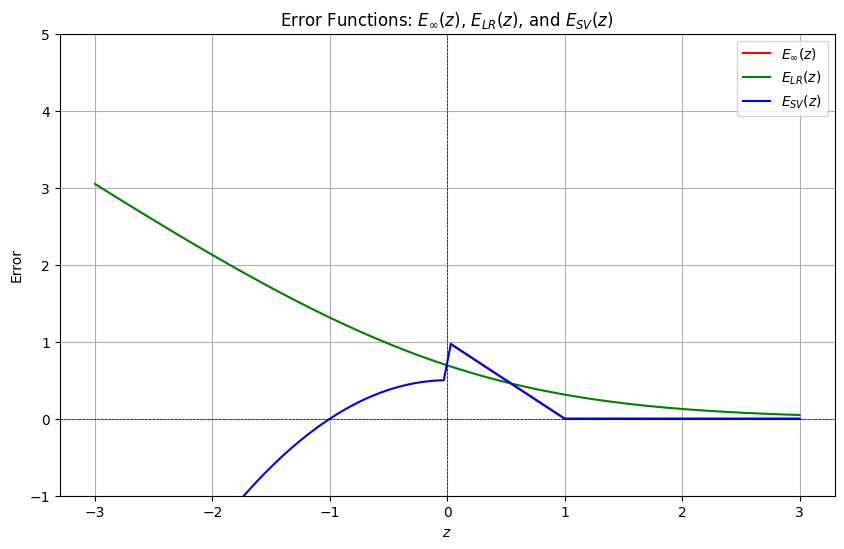
\includegraphics[width=0.68\textwidth]{2_1_d_output.png}  
    \label{fig:Three erroe functions}
\end{figure}

We can see that:
\begin{itemize}
    \item \(E_\infty(z)\): It exhibits a hard threshold; any misclassification incurs an infinite penalty. This is ideal for a clear margin but may not be suitable for noisy data.
    \item \(E_{LR}(z)\): It is smooth and continuous, which allows for a softer transition between correct and incorrect classifications. This smoothness can help the optimization process, leading to better convergence properties.
    \item \(E_{SV}(z)\): It balances balances misclassifications and model complexity. The quadratic penalty for \(z < 0\) help avoid extreme penalities while still enforcing the margin constraints.
\end{itemize}

If the error functions are replaced with other functions, several outcomes may arise:

\begin{itemize}
    \item \textbf{Loss of Robustness}: Using an overly aggressive loss function (like a hard-margin SVM) may lead to poor generalization on noisy or overlapping datasets, resulting in overfitting.
    \item \textbf{Convergence Issues}: Non-smooth functions could lead to difficulties in optimization, causing convergence problems or slow training.
    \item \textbf{Behavior in Overlapping Data}: For functions that do not adequately penalize misclassifications, such as squared error loss in classification tasks, the model may not handle overlap well, potentially leading to high error rates.
    \item \textbf{Interpretability and Application}: Different functions might have different interpretability and applications. For example, soft-margin SVM and logistic regression can be interpreted probabilistically, whereas a hard-margin approach may not.
\end{itemize}

\newpage

\section*{Problem 2.2: Naive Bayes Parameter Learning}

We are given a dataset \(\{(x^{(i)}, y^{(i)}), i = 1, 2, \dots, m\}\) where each \(x^{(i)}\) is an \(n\)-dimensional vector, with each element \(x_j^{(i)} \in \{0, 1\}\), and the labels \(y^{(i)} \in \{0, 1\}\).We have known the following model for Naive Bayes classification:

\(y^{(i)}\) follows a Bernoulli distribution:
\[
    y^{(i)} \sim \text{Bernoulli}(\phi_y)
\]

Given \(y^{(i)} = b\), the features \(x_j^{(i)}\) are independent and follow Bernoulli distributions:
\[
    x_j^{(i)} | y^{(i)} = b \sim \text{Bernoulli}(\phi_{j|y=b}), \quad b = 0, 1
\]

The joint probability distribution of a single data point \((x^{(i)}, y^{(i)})\) is:
\[
  p(x^{(i)}, y^{(i)} | \phi_y, \phi_{j|y=b}) = p(y^{(i)} | \phi_y) \cdot \prod_{j=1}^n p(x_j^{(i)} | y^{(i)}, \phi_{j|y=b})
\]

Specifically:
  
\begin{itemize}
    \item \(p(y^{(i)} | \phi_y) = \phi_y^{y^{(i)}} (1 - \phi_y)^{1 - y^{(i)}}\)
    \item \(p(x_j^{(i)} | y^{(i)} = b, \phi_{j|y=b}) = \phi_{j|y=b}^{x_j^{(i)}} (1 - \phi_{j|y=b})^{1 - x_j^{(i)}}\)
\end{itemize}

Thus, the joint probability can be written as:
\[
    p(x^{(i)}, y^{(i)} | \phi_y, \phi_{j|y=b}) = \phi_y^{y^{(i)}} (1 - \phi_y)^{1 - y^{(i)}} \cdot \prod_{j=1}^n \phi_{j|y=y^{(i)}}^{x_j^{(i)}} (1 - \phi_{j|y=y^{(i)}})^{1 - x_j^{(i)}}
\]

The likelihood function for the entire dataset is the product of the joint probabilities for all data points:
\[
    L(\phi_y, \phi_{j|y=b}) = \prod_{i=1}^m p(x^{(i)}, y^{(i)} | \phi_y, \phi_{j|y=b}) = \prod_{i=1}^m \left( \phi_y^{y^{(i)}} (1 - \phi_y)^{1 - y^{(i)}} \prod_{j=1}^n \phi_{j|y=y^{(i)}}^{x_j^{(i)}} (1 - \phi_{j|y=y^{(i)}})^{1 - x_j^{(i)}} \right)
\]

To simplify calculations, we take the logarithm of the likelihood function:
\[
\log L(\phi_y, \phi_{j|y=b}) = \sum_{i=1}^m \left( y^{(i)} \log \phi_y + (1 - y^{(i)}) \log (1 - \phi_y) \right)
\]
\[
+ \sum_{i=1}^m \sum_{j=1}^n \left( x_j^{(i)} \log \phi_{j|y=y^{(i)}} + (1 - x_j^{(i)}) \log (1 - \phi_{j|y=y^{(i)}}) \right)
\]

We now compute the MLE of the parameters by taking the derivative of the log-likelihood function and setting it to zero.

\begin{quote}
    \textbf{For \(\phi_y\):}
    \[
        \frac{\partial \log L}{\partial \phi_y} = \sum_{i=1}^m \left( \frac{y^{(i)}}{\phi_y} - \frac{1 - y^{(i)}}{1 - \phi_y} \right)
    \]

    Setting this to zero, we obtain the MLE for \(\phi_y\):

    \[
        \hat{\phi}_y = \frac{1}{m} \sum_{i=1}^m y^{(i)}
    \]
    
    This is the proportion of samples where \(y = 1\).

    \textbf{For \(\phi_{j|y=b}\):}

    \[
        \frac{\partial \log L}{\partial \phi_{j|y=b}} = \sum_{i=1}^m \left( \frac{x_j^{(i)}}{\phi_{j|y=b}} - \frac{1 - x_j^{(i)}}{1 - \phi_{j|y=b}} \right) 1\{y^{(i)} = b\}
    \]
    \[
        \hat{\phi}_{j|y=b} = \frac{\sum_{i=1}^m 1\{y^{(i)} = b\} x_j^{(i)}}{\sum_{i=1}^m 1\{y^{(i)} = b\}}
    \]

    This is the proportion of times feature \(x_j = 1\) when \(y = b\). 

\end{quote}

The maximum likelihood estimates for the parameters are:

\begin{quote}
    \[
    \hat{\phi}_y = \frac{1}{m} \sum_{i=1}^m y^{(i)}
    \]
    \[\hat{\phi}_{j|y=b} = \frac{\sum_{i=1}^m 1\{y^{(i)} = b\} x_j^{(i)}}{\sum_{i=1}^m 1\{y^{(i)} = b\}}
    \]
\end{quote}

\newpage

\section*{Problem 2.3: Comparison of Genetrative and Discriminative Models}

\subsection*{(a) Parameter Estimation for GDA}

We are asked to derive the parameter estimation for Gaussian Discriminant Analysis (GDA) with a shared covariance matrix. The setup is as follows:

\begin{itemize}
    \item $ y \sim \text{Bernoulli}(\phi) $
    \item $ x | y = 0 \sim \mathcal{N}(\mu_0, \Sigma) $
    \item $ x | y = 1 \sim \mathcal{N}(\mu_1, \Sigma) $
\end{itemize}

To estimate the parameters $\mu_0$, $\mu_1$, $\Sigma$, and $\phi$, we use the maximum likelihood method.

\begin{itemize}
    \item \textbf{Estimate $\phi$}: The probability of the label $y = 1$ is estimated by the fraction of positive labels:
    \[
    \hat{\phi} = \frac{1}{n} \sum_{i=1}^n y^{(i)}
    \]

    \item \textbf{Estimate $\mu_0$ and $\mu_1$}: The mean vectors $\mu_0$ and $\mu_1$ are the empirical means of the samples that have $y = 0$ and $y = 1$ respectively:
    \[
    \hat{\mu}_0 = \frac{\sum_{i: y^{(i)} = 0} x^{(i)}}{\sum_{i=1}^n 1\{y^{(i)} = 0\}}
    \]
    \[
    \hat{\mu}_1 = \frac{\sum_{i: y^{(i)} = 1} x^{(i)}}{\sum_{i=1}^n 1\{y^{(i)} = 1\}}
    \]
    
    \item \textbf{Estimate $\Sigma$}: The shared covariance matrix $\Sigma$ is estimated by pooling the covariance across both classes:
    \[
    \hat{\Sigma} = \frac{1}{n} \sum_{i=1}^n \left( x^{(i)} - \mu_{y^{(i)}} \right)\left( x^{(i)} - \mu_{y^{(i)}} \right)^T
    \]
    where $\mu_{y^{(i)}}$ is $\mu_0$ if $y^{(i)} = 0$, and $\mu_1$ if $y^{(i)} = 1$.
\end{itemize}

\subsection*{(b) Compute for the Parameters}

The dataset provided is:
\[
x^{(1)} = \begin{pmatrix} 1 \\ 2 \end{pmatrix}, \quad y^{(1)} = 0
\]
\[
x^{(2)} = \begin{pmatrix} 2 \\ 3 \end{pmatrix}, \quad y^{(2)} = 0
\]
\[
x^{(3)} = \begin{pmatrix} 3 \\ 4 \end{pmatrix}, \quad y^{(3)} = 1
\]
\[
x^{(4)} = \begin{pmatrix} 4 \\ 5 \end{pmatrix}, \quad y^{(4)} = 1
\]

\begin{itemize}
    \item \textbf{Estimate $\phi$}:
    \[
    \hat{\phi} = \frac{1}{4} \left( y^{(1)} + y^{(2)} + y^{(3)} + y^{(4)} \right) = \frac{1}{4} \left( 0 + 0 + 1 + 1 \right) = \frac{1}{2}
    \]

    \item \textbf{Estimate $\mu_0$}:
    \[
    \hat{\mu}_0 = \frac{x^{(1)} + x^{(2)}}{2} = \frac{1}{2} \left( \begin{pmatrix} 1 \\ 2 \end{pmatrix} + \begin{pmatrix} 2 \\ 3 \end{pmatrix} \right) = \begin{pmatrix} 1.5 \\ 2.5 \end{pmatrix}
    \]

    \item \textbf{Estimate $\mu_1$}:
    \[
    \hat{\mu}_1 = \frac{x^{(3)} + x^{(4)}}{2} = \frac{1}{2} \left( \begin{pmatrix} 3 \\ 4 \end{pmatrix} + \begin{pmatrix} 4 \\ 5 \end{pmatrix} \right) = \begin{pmatrix} 3.5 \\ 4.5 \end{pmatrix}
    \]

    \item \textbf{Estimate $\Sigma$}: First, we calculate the covariance terms. For the class $y = 0$:
    \[
    (x^{(1)} - \mu_0) = \begin{pmatrix} 1 \\ 2 \end{pmatrix} - \begin{pmatrix} 1.5 \\ 2.5 \end{pmatrix} = \begin{pmatrix} -0.5 \\ -0.5 \end{pmatrix}
    \]
    \[
    (x^{(2)} - \mu_0) = \begin{pmatrix} 2 \\ 3 \end{pmatrix} - \begin{pmatrix} 1.5 \\ 2.5 \end{pmatrix} = \begin{pmatrix} 0.5 \\ 0.5 \end{pmatrix}
    \]

    For the class $y = 1$:
    \[
    (x^{(3)} - \mu_1) = \begin{pmatrix} 3 \\ 4 \end{pmatrix} - \begin{pmatrix} 3.5 \\ 4.5 \end{pmatrix} = \begin{pmatrix} -0.5 \\ -0.5 \end{pmatrix}
    \]
    \[
    (x^{(4)} - \mu_1) = \begin{pmatrix} 4 \\ 5 \end{pmatrix} - \begin{pmatrix} 3.5 \\ 4.5 \end{pmatrix} = \begin{pmatrix} 0.5 \\ 0.5 \end{pmatrix}
    \]

    Now calculate the covariance matrix:
    \[
    \Sigma = \frac{1}{4} \left( \begin{pmatrix} -0.5 \\ -0.5 \end{pmatrix} \begin{pmatrix} -0.5 & -0.5 \end{pmatrix} + \begin{pmatrix} 0.5 \\ 0.5 \end{pmatrix} \begin{pmatrix} 0.5 & 0.5 \end{pmatrix} + \begin{pmatrix} -0.5 \\ -0.5 \end{pmatrix} \begin{pmatrix} -0.5 & -0.5 \end{pmatrix} + \begin{pmatrix} 0.5 \\ 0.5 \end{pmatrix} \begin{pmatrix} 0.5 & 0.5 \end{pmatrix} \right)
    \]
    \[
    = \begin{pmatrix} 0.25 & 0.25 \\ 0.25 & 0.25 \end{pmatrix}
    \]
\end{itemize}
The computed parameters for this dataset are:

\begin{itemize}
    \item $\hat{\phi} = 0.5$
    \item $\hat{\mu}_0 = \begin{pmatrix} 1.5 \\ 2.5 \end{pmatrix}$
    \item $\hat{\mu}_1 = \begin{pmatrix} 3.5 \\ 4.5 \end{pmatrix}$
    \item $\hat{\Sigma} = \begin{pmatrix} 0.25 & 0.25 \\ 0.25 & 0.25 \end{pmatrix}$
\end{itemize}
\newpage
\subsection*{(c) Decision Boundary for LDA}

The decision boundary is derived by finding the point where the probabilities of the two classes are equal, i.e., $P(y=0|x)=P(y=1|x)$.Since both classes follow Gaussian distributions with equal covariance matrices, the decision rule simplifies to:

\[
    \hat y=\hat{y} = \arg\max_y P(y | x) = \arg\max_y \log P(x | y) + \log P(y)
\]

This leads to the decision boundary equation:

\[
x^T \Sigma^{-1} (\mu_0 - \mu_1) = \frac{1}{2} (\mu_0^T \Sigma^{-1} \mu_0 - \mu_1^T \Sigma^{-1} \mu_1) + \log \left( \frac{\phi}{1 - \phi} \right)
\]

\subsection*{(d) Decision Boundaries Comparion of LDA and LR}

\subsubsection*{a. LDA Decision Boundary}

From the part (c),we derived that the decision boundary for LDA is given by:

\[
    x^T \Sigma^{-1} (\mu_0 - \mu_1) = \frac{1}{2} (\mu_0^T \Sigma^{-1} \mu_0 - \mu_1^T \Sigma^{-1} \mu_1) + \log \left( \frac{\phi}{1 - \phi} \right)
\]

When \(\Sigma=I\)(Identity Mrix),the decision boundary simplifies to:

\[
    x^T (\mu_0 - \mu_1) = \frac{1}{2} (\mu_0^T \mu_0 - \mu_1^T \mu_1) + \log \left( \frac{\phi}{1 - \phi} \right)
\]

\subsubsection*{b. LR Decision Boundary}

Logistic regression models the conditional probability \(P(y = 1 | x)\) directly using a sigmoid function:

\[
    P(y = 1 | x) = \frac{1}{1 + \exp\left(- \theta^T x \right)}
\]

The decision boundary is found by solving:

\[
    P(y = 1 | x) = P(y = 0 | x)
\]

or equivalently:

\[
    \theta^T x = 0
\]

\subsubsection*{c. Comparison}

\begin{itemize}
    \item Both LDA (with \(\Sigma = I\)) and LR have \textbf{linear decision boundaries}.
    \item LDA assumes a Gaussian distribution for the data (generative approach), while Logistic Regression does not make any distributional assumptions and models the posterior probabilities directly (discriminative approach).
    \item If \(\Sigma \neq I\), the decision boundary for LDA can still be linear but may become more complex depending on the covariance structure, whereas Logistic Regression will always produce a linear boundary.
\end{itemize}

\subsection*{(e) LDA vs LR on Small Datasets}

\subsubsection*{a. LR on Small Datasets}

\begin{itemize}
    \item Logistic Regr ession is a \textbf{discriminative model}, which means it directly models \(P(y | x)\) without making assumptions about the underlying distribution of the data.
    \item On small datasets, this can be problematic because logistic regression might not have enough data to accurately estimate \(P(y | x)\) without overfitting. It lacks the \textbf{regularizing effect} of modeling the data's distribution, which a generative model provides.
\end{itemize}

\subsubsection*{b. LDA on Small Datasets}

\begin{itemize}
    \item LDA is a \textbf{generative model}, meaning it models the joint distribution \(P(x, y)\), specifically \(P(x | y)\) and \(P(y)\). 
    \item LDA benefits from making stronger assumptions about the data (e.g., Gaussian distribution with shared covariance).
\end{itemize}

\subsubsection*{c. Why Generative Models Might Perform Better}

\begin{itemize}
    \item \textbf{With small datasets}, the limited amount of data can make it difficult for discriminative models like logistic regression to accurately learn the conditional probabilities.
    \item \textbf{Generative models}, such as LDA, can perform better because they make use of the \textbf{entire data distribution}, imposing structure via assumptions like Gaussianity. This helps stabilize predictions, even with small data.
\end{itemize}

\end{document}
